%! Author = dmitriy
%! Date = 9/15/23

% Preamble
\documentclass[14pt]{extreport}
\usepackage{gost}
\usepackage{ragged2e}

%\usepackage{blindtext}
\justifying
\renewcommand{\thefigure}{\arabic{figure}}
\renewcommand{\thetable}{\arabic{table}}

\begin{document}
    \pagestyle{empty}
    
\includepdf[pages=-,pagecommand={}]{title.pdf}
    \pagestyle{plain}
    \tableofcontents

    \intro Лабораторная работа №3 направлена на анализ и оптимизацию отношений, полученных в результате построения предметной области, описанной в лабораторной работе №1. Задачи включают в себя описание функциональных зависимостей для полученной схемы, приведение отношений в 3NF и BCNF, а также анализ изменений в функциональных зависимостях после преобразований. Дополнительно, рассматриваются вопросы денормализации схемы и предлагается подробное описание необходимых денормализаций.

    \chapter{Текст задания:}
        Для отношений, полученных при построении предметной области из лабораторной работы №1, выполните следующие действия:
        \begin{enumerate}
        \item Опишите функциональные зависимости для отношений полученной схемы (минимальное множество);
        \item Приведите отношения в 3NF (как минимум). Постройте схему на основеNF (как минимум).
        \item Опишите изменения в функциональных зависимостях, произошедшие после преобразования в 3NF (как минимум). Постройте схему на основеNF;
        \item Преобразуйте отношения в BCNF. Докажите, что полученные отношения представлены в BCNF. Если ваша схема находится уже в BCNF, докажите это;
        \item Какие денормализации будут полезны для вашей схемы? Приведите подробное описание.
        \item Придумайте триггер и связанную с ним функцию, относящиеся к вашей предметной области, согласуйте их с преподавателем и реализуйте на языке PL/pgSQL.
        \end{enumerate}

        \bigskip

    Предметная область:

    Ян Малкольм лежал на спине, кожа у него была бледно-серого цвета, ротшироко открыт. Дыхание вырывалось изо рта с жуткими хрипами. Малдунпротянул Дженнаро фонарь и наклонился, осматривая пострадавшего.

\begin{landscape}
    \chapter{Функциональные зависимости}
        \begin{tabular}{|c|c|}
            \hline
            Patients & patient\_id $\rightarrow$ name, position, skin\_color, condition\\ \hline
            MedicalStaff & staff\_id $\rightarrow$ name, role \\ \hline
            Instruments & instrument\_id $\rightarrow$ name \\ \hline
            InstrumentTransfer & \begin{tabular}{c}
                                     transfer\_id $\rightarrow$ from\_staff\_id, to\_staff\_id, instrument\_id, transfer\_time \\


                                \end{tabular} \\ \hline
            Examintaions & \begin{tabular}{c}
                               examination\_id $\rightarrow$ patient\_id, staff_id, examination\_time \\
                               patient\_id, staff\_id, examination\_time $\rightarrow$ examination\_id
                           \end{tabular} \\

            \hline
        \end{tabular}
\end{landscape}

\chapter{Нормализованная модель}
    \section{3-я нормальная форма}
    База данных уже находится в 3-й нормальной форме.

    Доказательство:
        \begin{itemize}
            \item Patients \begin{itemize}
                      \item 1NF: Все атрибуты являются атомарными, и нет составных значений.
                      \item 2NF: Нет составных первичных ключей, так что 2NF автоматически удовлетворяется.
                      \item 3NF: Нет транзитивных зависимостей, так как все атрибуты зависят только от первичного ключа patient\_id.
            \end{itemize}

            \item MedicalStaff \begin{itemize}
                      \item 1NF: Все атрибуты атомарны.
                      \item 2NF: Все атрибуты зависят от полного первичного ключа staff\_id.
                      \item 3NF: Нет транзитивных зависимостей.
            \end{itemize}

            \item Instruments \begin{itemize}
                      \item 1NF: Все атрибуты атомарны.
                      \item 2NF: Все атрибуты зависят от полного первичного ключа instrument\_id.
                      \item 3NF: Нет транзитивных зависимостей.
            \end{itemize}

            \item InstrumentTransfer \begin{itemize}
                      \item 1NF: Все атрибуты атомарны.
                      \item 2NF: Все атрибуты зависят от полного первичного ключа transfer\_id.
                      \item 3NF: Нет транзитивных зависимостей.
            \end{itemize}

            \item Examinations \begin{itemize}
                      \item 1NF: Все атрибуты атомарны.
                      \item 2NF: Все атрибуты зависят от полного первичного ключа examination\_id.
                      \item 3NF: Нет транзитивных зависимостей.
            \end{itemize}
        \end{itemize}

            \begin{landscape}
                \begin{figure}[h]
                    \centering
                    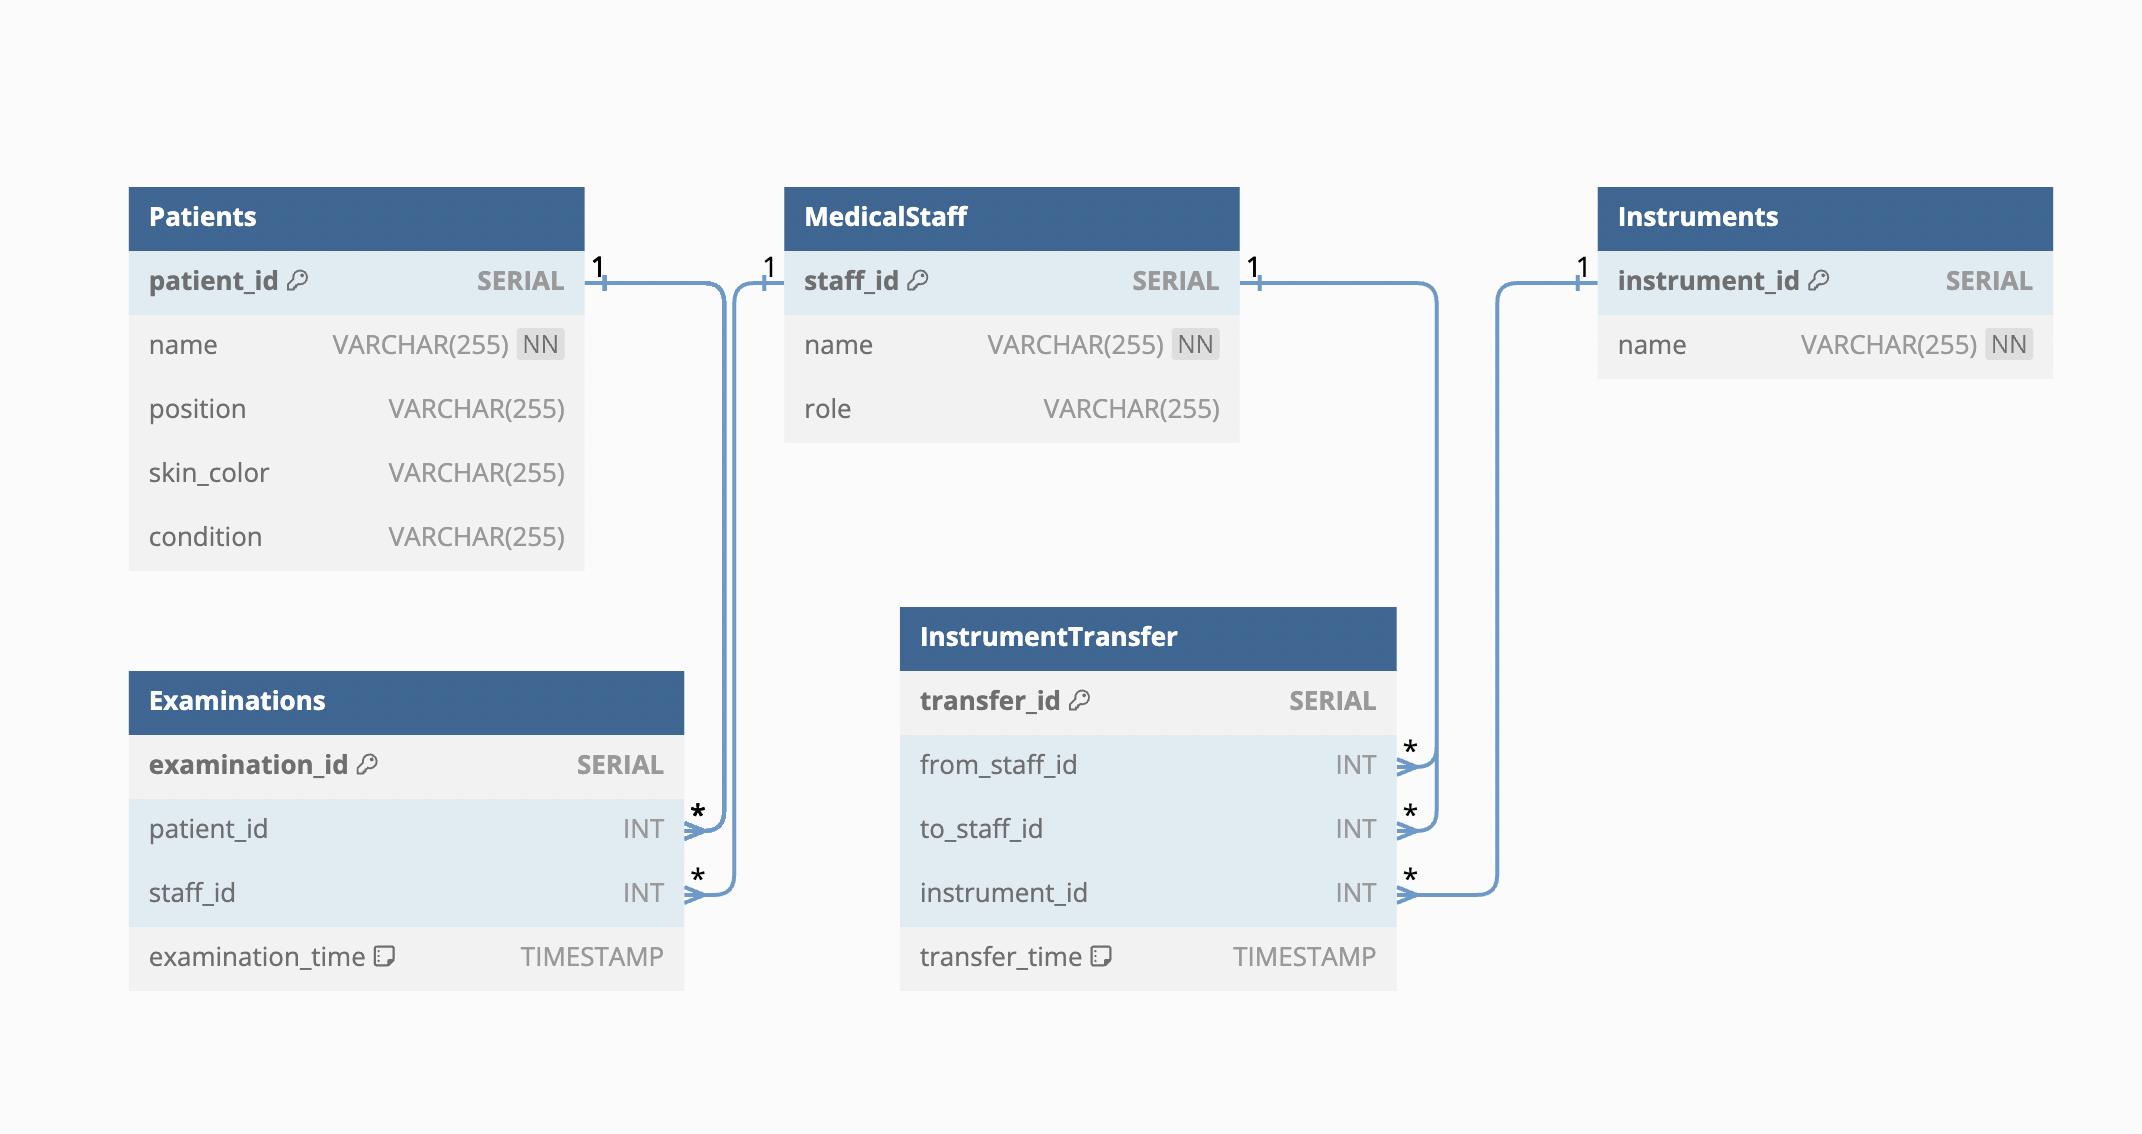
\includegraphics[width=21cm]{ddl.png}
                \end{figure}
                \end{landscape}


    \section{BCNF}
            База данных соответствует Boyce-Codd Normal Form, так как каждая таблица удовлетворяет критериям BCNF:

            \begin{enumerate}[label=\arabic*.]
                \item \textbf{Patients:}
                \begin{itemize}
                    \item $\text{patient\_id} \rightarrow \text{name, position, skin\_color, condition}$ (BCNF, так как $\text{patient\_id}$ - первичный ключ).
                \end{itemize}

                \item \textbf{MedicalStaff:}
                \begin{itemize}
                    \item $\text{staff\_id} \rightarrow \text{name, role}$ (BCNF, так как $\text{staff\_id}$ - первичный ключ).
                \end{itemize}

                \item \textbf{Instruments:}
                \begin{itemize}
                    \item $\text{instrument\_id} \rightarrow \text{name}$ (BCNF, так как $\text{instrument\_id}$ - первичный ключ).
                \end{itemize}

                \item \textbf{InstrumentTransfer:}
                \begin{itemize}
                    \item $\text{transfer\_id} \rightarrow \text{from\_staff\_id, to\_staff\_id, instrument\_id, transfer\_time}$
                    \item $\text{from\_staff\_id, to\_staff\_id, instrument\_id} \rightarrow \text{transfer\_id}$
                    \item $\text{instrument\_id} \rightarrow \text{from\_staff\_id, to\_staff\_id}$ (BCNF, так как $\text{transfer\_id}$ - первичный ключ).
                \end{itemize}

                \item \textbf{Examinations:}
                \begin{itemize}
                    \item $\text{examination\_id} \rightarrow \text{patient\_id, staff\_id, examination\_time}$ (BCNF, так как $\text{examination\_id}$ - первичный ключ).
                \end{itemize}
            \end{enumerate}

    \chapter{Денормализация}
    \begin{itemize}
        \item Создание таблицы для отображения информации о пациенте, объединяющей атрибуты из таблицы Patients и Examinations, чтобы избежать необходимости объединения таблиц при частых запросах на отображение данных о пациентах и их обследованиях.
        \item Добавление атрибута current\_staff\_id в таблицу Instruments, который содержит информацию о текущем владельце инструмента. Это позволит избежать дополнительных JOIN-операций при поиске текущего владельца инструмента.
        \item Добавление атрибута last\_examination\_time в таблицу Patients, который содержит информацию о времени последнего обследования для каждого пациента. Это позволит избежать JOIN-операции при поиске последнего обследования.
        \item Добавление атрибута last\_instrument\_id в таблицу MedicalStaff, который содержит информацию о последнем использованном инструменте для каждого медицинского персонала. Это избавляет от необходимости JOIN при поиске последнего использованного инструмента.
    \end{itemize}

    \chapter{Функция и триггер на языке PL/pgSQL}
    Была реализована функция, которая при изменении цвета кожи пациента на normal, автоматически устанавливает состояние пациента на good.

        \begin{verbatim}
CREATE OR REPLACE FUNCTION update_condition_on_skin_color()
RETURNS TRIGGER AS $$
BEGIN
  IF NEW.skin_color = 'normal' THEN
    UPDATE Patients
    SET condition = 'good'
    WHERE patient_id = NEW.patient_id;
  END IF;
  RETURN NEW;
END;
$$ LANGUAGE plpgsql;

CREATE TRIGGER after_update_skin_color
AFTER UPDATE OF skin_color ON Patients
FOR EACH ROW
EXECUTE FUNCTION update_condition_on_skin_color();

            \end{verbatim}
    \conclusions Лабораторная работа проведена успешно, и результаты оптимизации схемы отношений подтверждают ее соответствие требованиям 3NF и BCNF. Проанализированы функциональные зависимости, а также предложены денормализации для оптимизации производительности. Кроме того, разработаны и реализованы триггер и связанная с ним функция на языке PL/pgSQL, соответствующие предметной области, после их предварительного согласования с преподавателем. Полученные результаты подчеркивают важность проектирования эффективных баз данных для обеспечения оптимальной работы системы.
\end{document}